\chapter{ニュースアンカーの発話検出実験}
\label{chapter:get_anchor}
本章では、発話区間結合を行い、結合した発話区間から抽出したi-vectorを用いてニュースアンカーの発話検出を行った。

\section{実験条件}
i-vectorの抽出には、ALIZEとLIR RAL\cite{alize}を用いる。i-vectorの抽出に使用するUBMモデルの学習には読み上げ音声\cite{ATR}を使用する。読み上げ音声に収録されている各発話データからi-vectorを抽出する。発話データから抽出する音響特徴パラメータを表\ref{iv_feature2}に示す。また混合数は32とした。\par

\begin{table}[H]
  \begin{center}
    \caption{使用する音響特徴パラメータ \label{iv_feature2}}
    \begin{tabular}{|c||c|} \hline
      特徴量 & 次元数\\ \hline
      MFCC & 19  \\ 
      POW & 1  \\ 
      $\Delta$MFCC & 19 \\ 
      $\Delta$POW & 1 \\ 
      $\Delta\Delta$MFCC & 19 \\ 
      $\Delta\Delta$POW & 1 \\ \hline
      計 & 60 \\ \hline
    \end{tabular}
  \end{center}
\end{table}

\vspace{0.2in}\noindent{\textbf{\underline{評価データ}}}\par
「音声」の音源ラベルと発話の書き起こしが付与されているニュース番組5番組分を用いてニュースアンカーの発話区間検出を行う。ニュース番組音声の詳細を表\ref{table:test_detail}に示す。また、ニュース番組5番組分に音源識別を用いて検出した発話区間の詳細を表\ref{table:num_of_anchor}に示す。音源識別の詳細は付録\ref{section:devide_audio}に記載する。

\begin{table}[H]
  \begin{center}
    \caption{評価データの詳細 \label{table:test_detail}}
    \begin{tabular}{|c||c|c|c|} \hline
ニュースID & ニュースアンカー数 & 発話区間数 & ニュースアンカーの発話区間数 \\ \hline
ニュース1  & 1 & 114 & 69 \\ \hline
ニュース2  & 2 & 194 & 76 \\ \hline
ニュース3  & 2 & 214 & 133 \\ \hline
ニュース4  & 2 & 195 & 127 \\ \hline
ニュース5  & 2 & 203 & 139 \\ \hline
    \end{tabular}
  \end{center}
\end{table}

\begin{table}[H]
  \begin{center}
    \caption{検出した発話区間数とニュースアンカーの発話区間数 \label{table:num_of_anchor}}
    \begin{tabular}{|c||c|c|} \hline
ニュースID & 発話区間数 & ニュースアンカーの発話区間数 \\ \hline
ニュース1  & 345   & 165 \\ \hline
ニュース2  & 519   & 149 \\ \hline
ニュース3  & 608   & 258 \\ \hline
ニュース4  & 518   & 219 \\ \hline
ニュース5  & 520   & 285 \\ \hline
    \end{tabular}
  \end{center}
\end{table}

\section{i-vectorの抽出精度向上のための発話区間結合手法}
\label{chapter:prob_method}
i-vectorは発話ができるだけ長いほうが正確に話者の特徴を抽出することができる。そこで、時系列順に並んでいる発話区間のうち、前後の発話が同一話者である可能性が高い発話区間を結合、擬似的に長い発話を作成する。本稿では発話から抽出できるi-vectorに加えて、「発話の時間間隔」「発話環境」を考慮した2通りの手法で発話区間を結合した。図\ref{fig:indexing2}は本稿の提案手法を組み込んだインデックス付与までの流れである。

\begin{figure}[H]
  \begin{center}
    \includegraphics[scale=0.3]{./figure/indexing2.eps}
  \end{center}
  \caption{提案手法を組み込んだインデクシング手法 \label{fig:indexing2}}
\end{figure}

\subsection{発話の時間間隔を考慮した発話区間の結合手法}
\label{prob1}
同一話者が連続で発話する場合、間をおかずに次の発話を行うことが多い。そのため、発話区間と発話区間の間(非発話区間)が非常に短いとき、高い確率で同一話者の発話が行われていると考えられる。また、インタビューイや中継アナウンサーなど話者が切り替わった場合、ニュースの画面も切り替わるため非発話区間は長くなる。そこで本手法では、発話から抽出されるコサイン類似度が一定値以上を示し、かつ非発話区間が非常に短いとき、同一話者の発話と判別して発話区間を結合する。

\subsection{発話環境を考慮した発話区間の結合手法}
\label{prob2}
ニュース番組にはスタジオにいるアンカーのほか、台風の状況を中継する中継アナウンサー、騒音の中でインタビューを受けるインタビューイなどが存在する。そこで、アンカーから中継アナウンサー、インタビューイからアンカーなど話者が切り替わった場合、発話環境が変化することに着目した。本稿で使用する音源識別システムはニュース番組音声を「音声」「背景雑音」「音楽」「無音」のいずれかに分類する。そのため、「音声」以外の区間、つまり非発話区間の音源識別結果である「背景雑音」「音楽」「無音」の検出結果が変化した時、発話環境の変化したと識別することができる。そこで本手法では、発話から抽出されるコサイン類似度が一定値以上を示し、かつ発話環境が変化していないとき、同一話者として発話区間を結合する。\par


\section{i-vectorを用いたニュースアンカーの発話区間検出手法\cite{nozaki_gakuseikai}}
\label{section:clustering}
ニュースアンカーの発話区間検出のために、i-vectorを用いて話者クラスタを作成し、クラスタに含まれる発話が多いクラスタをニュースアンカーのクラスタとして発話区間を検出した。従来は話者クラスタの作成にk-meansが多く用いられていたが、ニュース番組ではニュースアンカー以外にインタビューイ(インタビューの受け手)や中継の有無によって話者数が大きく異なるため、
あらかじめクラスタ数を決定する必要があるk-meansクラスタリングを用いることは適切ではないと考えた。そのため、ニュースアンカーの発話数は非ニュースアンカーと比較して多いことと、i-vectorはベクトル空間上で話者ごとに局所的に分布することに着目た。多くの発話のi-vectorが局所的に分布している部分のみをクラスタリングすることで、同一ニュースアンカーの発話区間を検出する。\par
本手法では、2つの発話データのi-vectorのコサイン類似度が閾値$Th_{cos}$以上の場合、その2つの発話データの話者は同一話者であると仮定した。まず、全ての発話データ間のi-vectorのコサイン類似度を求める。次に、このコサイン類似度が閾値$Th_{cos}$以上となる発話データ数が最も多い発話データを同一アンカーの発話データ群$O$のセントロイドとし、閾値$Th_{cos}$以上(話者性が類似している)の全データをそのデータ群$O$の初期要素とする。一方、i-vectorを抽出する発話データの発声の抑揚が大きい場合、同一話者の発話間のi-vectorであってもコサイン類似度が閾値$Th_{cos}$以下になる場合がある。そこで、発話データ$u_i(\in O)$と発話データ群$O$の距離が一定距離以内であるとき、発話データ$u_i$は発話データ群$O$の要素として追加する。以上の手順を繰り返してクラスタリングを行い、クラスタに含まれる発話が一定数以下となった時、クラスタリングを終了する。\par

\section{実験方法}
同一話者の可能性が高い発話区間を結合し、結合した発話区間からi-vectorを再抽出した。次に、再抽出したi-vectorを用いてアンカーの発話区間検出を行った。発話区間の結合手法は以下の通りである。

\begin{itemize}
\item 手法1 : 前後の発話のi-vectorのコサイン類似度と発話の間隔情報を考慮して発話区間の結合する
\item 手法2 : 前後の発話のi-vectorのコサイン類似度と発話環境を考慮して発話区間の結合する
\item 手法3 : 前後の発話のi-vectorのコサイン類似度と発話の間隔情報、および発話環境を考慮して発話区間の結合する
\end{itemize}

また、音源識別によって得られた各発話区間から抽出したi-vectorを用いて、k-meansによるニュースアンカーの発話検出をBaseline1、先行研究\cite{nozaki_gakuseikai}によるニュースアンカーの発話検出をBaseline2として行う。k-meansは作成するクラスタ数によって結果が大きく異なるため、本実験では、kを5から30まで変更して実験を行う。


前後の発話区間を結合する際のi-vectorのコサイン類似度の閾値を表\ref{table:decide_thcos}に示す。ここで、$T$は発話区間の秒数である。これは、図\ref{fig:same_cos_hist}で示されるように、同一話者間の発話であっても発話の長さによってコサイン類似度の値が大きく異なり、図\ref{fig:same_cos_vari}で示されるように発話が短い時、同一話者間のi-vectorのコサイン類似度の標準偏差が非常に大きいためである。そのため、本実験では、3.5秒と7秒で閾値を変更し、発話区間の結合に用いた。

\begin{table}[H]
  \begin{center}
    \caption{発話区間の結合の閾値 \label{table:decide_thcos}}
    \begin{tabular}{|c||c|} \hline
時間条件 & コサイン類似度の閾値  \\ \hline
$T <$ 3.5 &  0.2 \\ \hline
3.5 $\leqq T <$ 7 &  0.6  \\ \hline
7 $\leqq T$ &  0.75 \\ \hline
    \end{tabular}
  \end{center}
\end{table}

手法1、および手法3で用いる非発話区間の長さの閾値$Th_{time}$は0.8秒から1.5秒までの範囲を0.1秒刻みで行う。これは、図\ref{fig:same_sp}で示されているように、同一話者間の非発話区間の長さが約1秒以下の割合が大きく、図\ref{fig:different_sp}より、異なる話者間の非発話区間の長さが2秒前後の割合が高いためである。\par
i-vectorを用いたニュースアンカーの発話区間検出におけるニュースアンカーか否かを判別する$Th_{cos}$は、先行研究\cite{nozaki_gakuseikai}と同様に0.5から0.8までの範囲を0.1刻みで変更して実験を行う。\par

\section{評価方法}
評価は、ニュースアンカーとして検出した発話の個数と、発話の時間の二通りで正解ラベルを比較して行う。

\begin{table}[H]
\begin{center}
    \caption{ニュースアンカーの発話区間の正誤判定 \label{table:clustering}}
\begin{tabular}{|c|c|c|c|l}
\cline{1-4}
\multicolumn{2}{|c|}{\multirow{2}{*}{}} & \multicolumn{2}{c|}{「発話者」のラベルが付与された発話区間} &  \\ \cline{3-4}
\multicolumn{2}{|c|}{}                  & ニュースアンカーの発話区間        & ニュースアンカー以外の発話区間        &  \\ \cline{1-4}
\multirow{2}{*}{判定結果}        & 正        & $TP$                  & $FP$                   &  \\ \cline{2-4}
& 誤        & $FN$                  & $TN$                   &  \\ \cline{1-4}
\end{tabular}
\end{center}
\end{table}

表\ref{table:clustering}に示すニュースアンカーの発話区間の正誤判定を行い、$P$(Precision)と$R$(Recall)を式\ref{calc:precision2}と式\ref{calc:recall2}のようにそれぞれ計算する。

\begin{equation}
\label{calc:precision2}
P = \frac{TP}{TP + FP},
\end{equation}

\begin{equation}
\label{calc:recall2}
R = \frac{TP}{TP + FN}.
\end{equation}

ここで$P$と$R$はそれぞれPrecision、Recallを表す。Precisionが高い値を取るとき、識別結果に含まれる「誤り」の割合が少ないことを示している。またRecallが高いとき、識別結果に「漏れ」が少ないことを示している。一般的に、Recallの高いシステムはPrecisionが低く、逆にPrecisionが高いシステムはRecallが低い傾向にある。評価指標が2つあるとどちらのシステムが優れているかの判断が難しいため、PrecisionとRecallの調和平均を取り、ひとつのスカラ値に変換したF-measureがある。

\begin{equation}
\label{calc:fmeasure}
F = \frac{2 \times P \times R}{P + R}. \notag
\end{equation}

\begin{comment}
また、検出したニュースアンカーの発話区間の時間の割合を式\ref{calc:anchor_acc}を用いて評価する。

\begin{equation}
\label{calc:anchor_acc}
Acc_{time} = \frac{検出したニュースアンカーの発話の時間数}{ニュースアンカーの発話の時間数}.
\end{equation}
\end{comment}

本実験では、評価指標としてPrecision、Recall、F-measureを用いる。

\section{実験結果}
noindent{\textbf{\underline{ニュースアンカーとして検出した発話の個数による評価}}}\par
$Th_{time}$を変更してニュースアンカーの発話の個数による発話検出精度が最も高いF-measureを示した条件の結果を図\ref{fig:result_anchor_baseline} $\sim$ 図\ref{fig:result_anchor_prob3}に示す。その他の条件の結果は付録\ref{other_result}で記載する。また、図\ref{baseline_fmeasure} $\sim$ 図\ref{prob3_fmeasure}に示された結果の中で、最も高いF-measureをとった$Th_{cos}$のときの各ニュース番組のニュースアンカーの発話検出精度とニュースアンカーとして検出したクラスタ数を表\ref{table:baseline_eachnews} $\sim$ 表\ref{table:prob3_eachnews}に示す。

\begin{figure}[H]
  \centering
    \begin{tabular}{c}
 
%----- recall -----
 
      \begin{minipage}{0.40\hsize}
        \centering
          \subfigure[Recall]{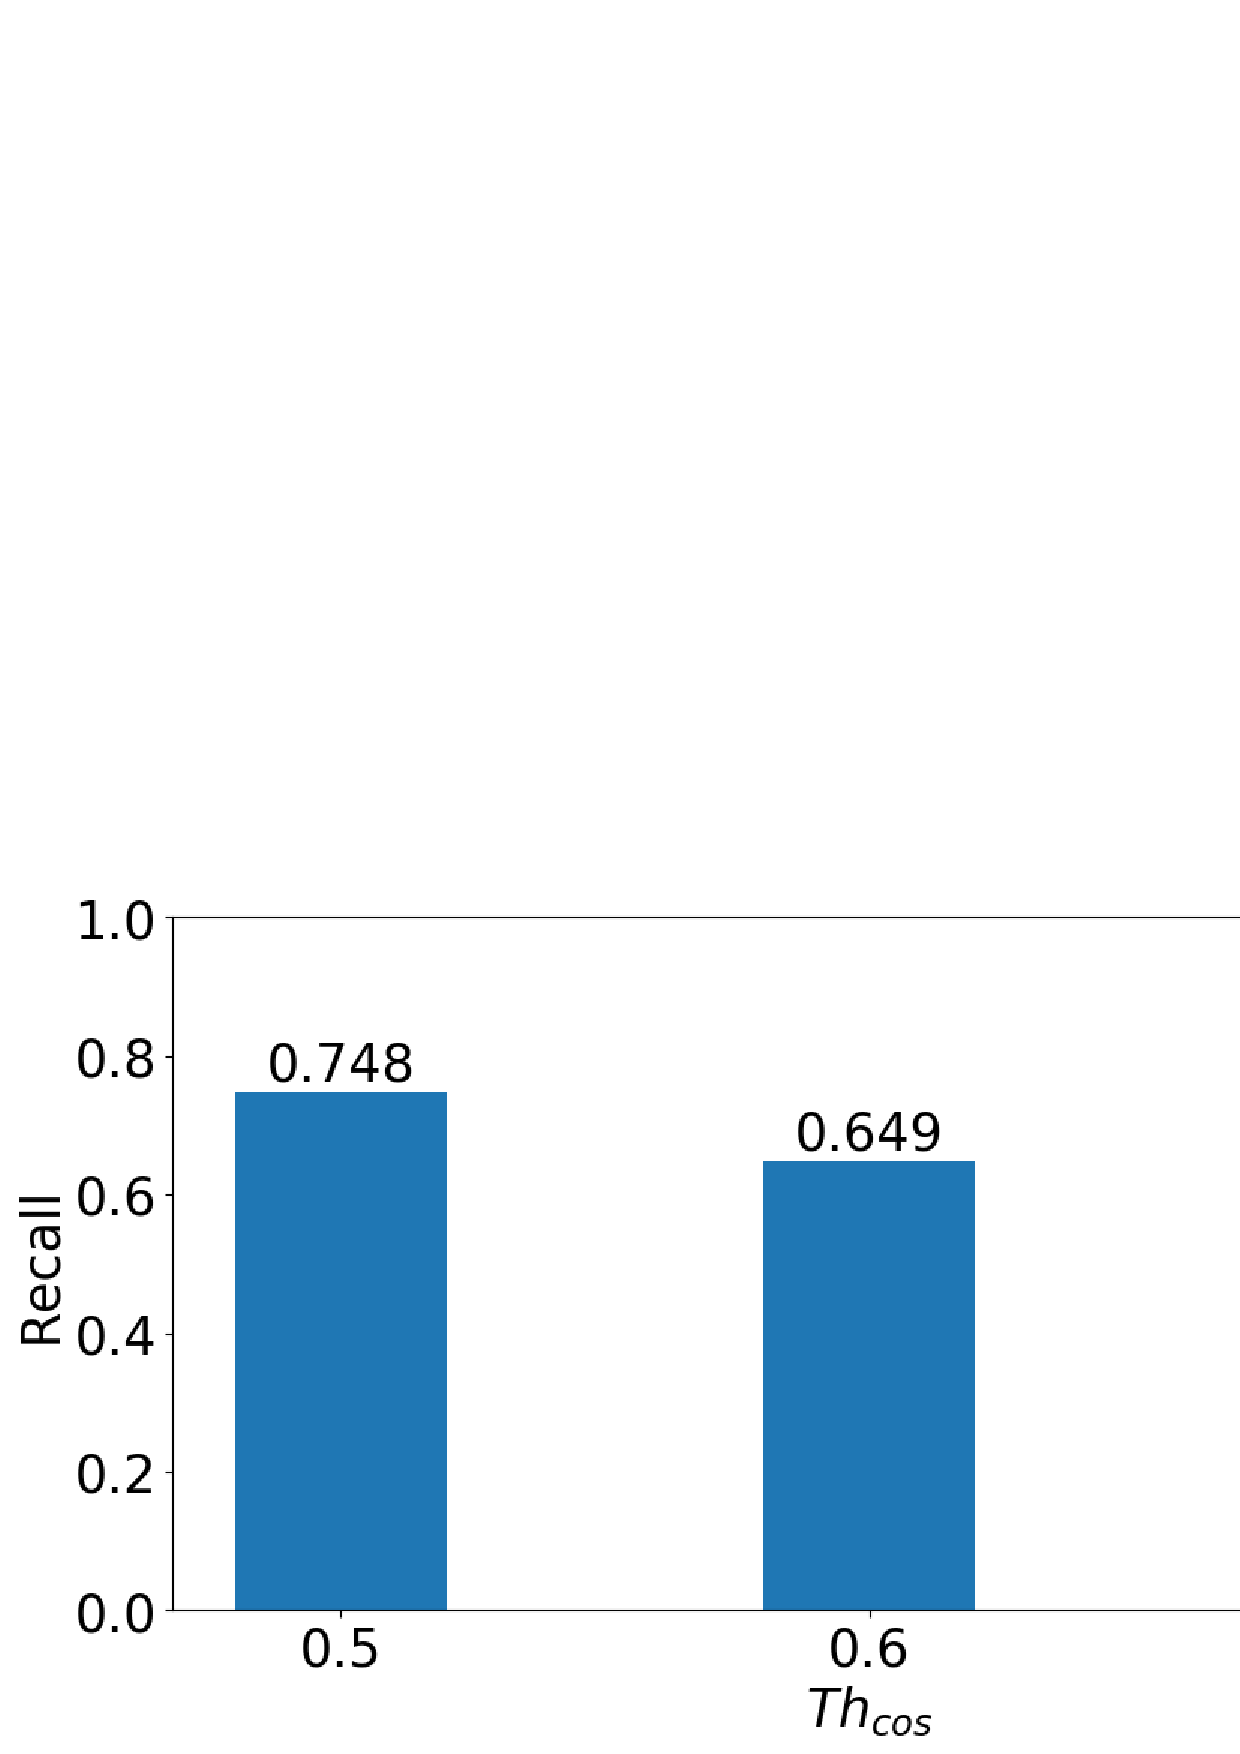
\includegraphics[keepaspectratio, scale=0.25]
                          {./figure/baseline_r.eps}}
      \end{minipage}

      \begin{minipage}{0.06\hsize}
        \hspace{0.5mm}
      \end{minipage}
 
%----- precision -----
 
      \begin{minipage}{0.40\hsize}
        \centering
          \subfigure[Precision]{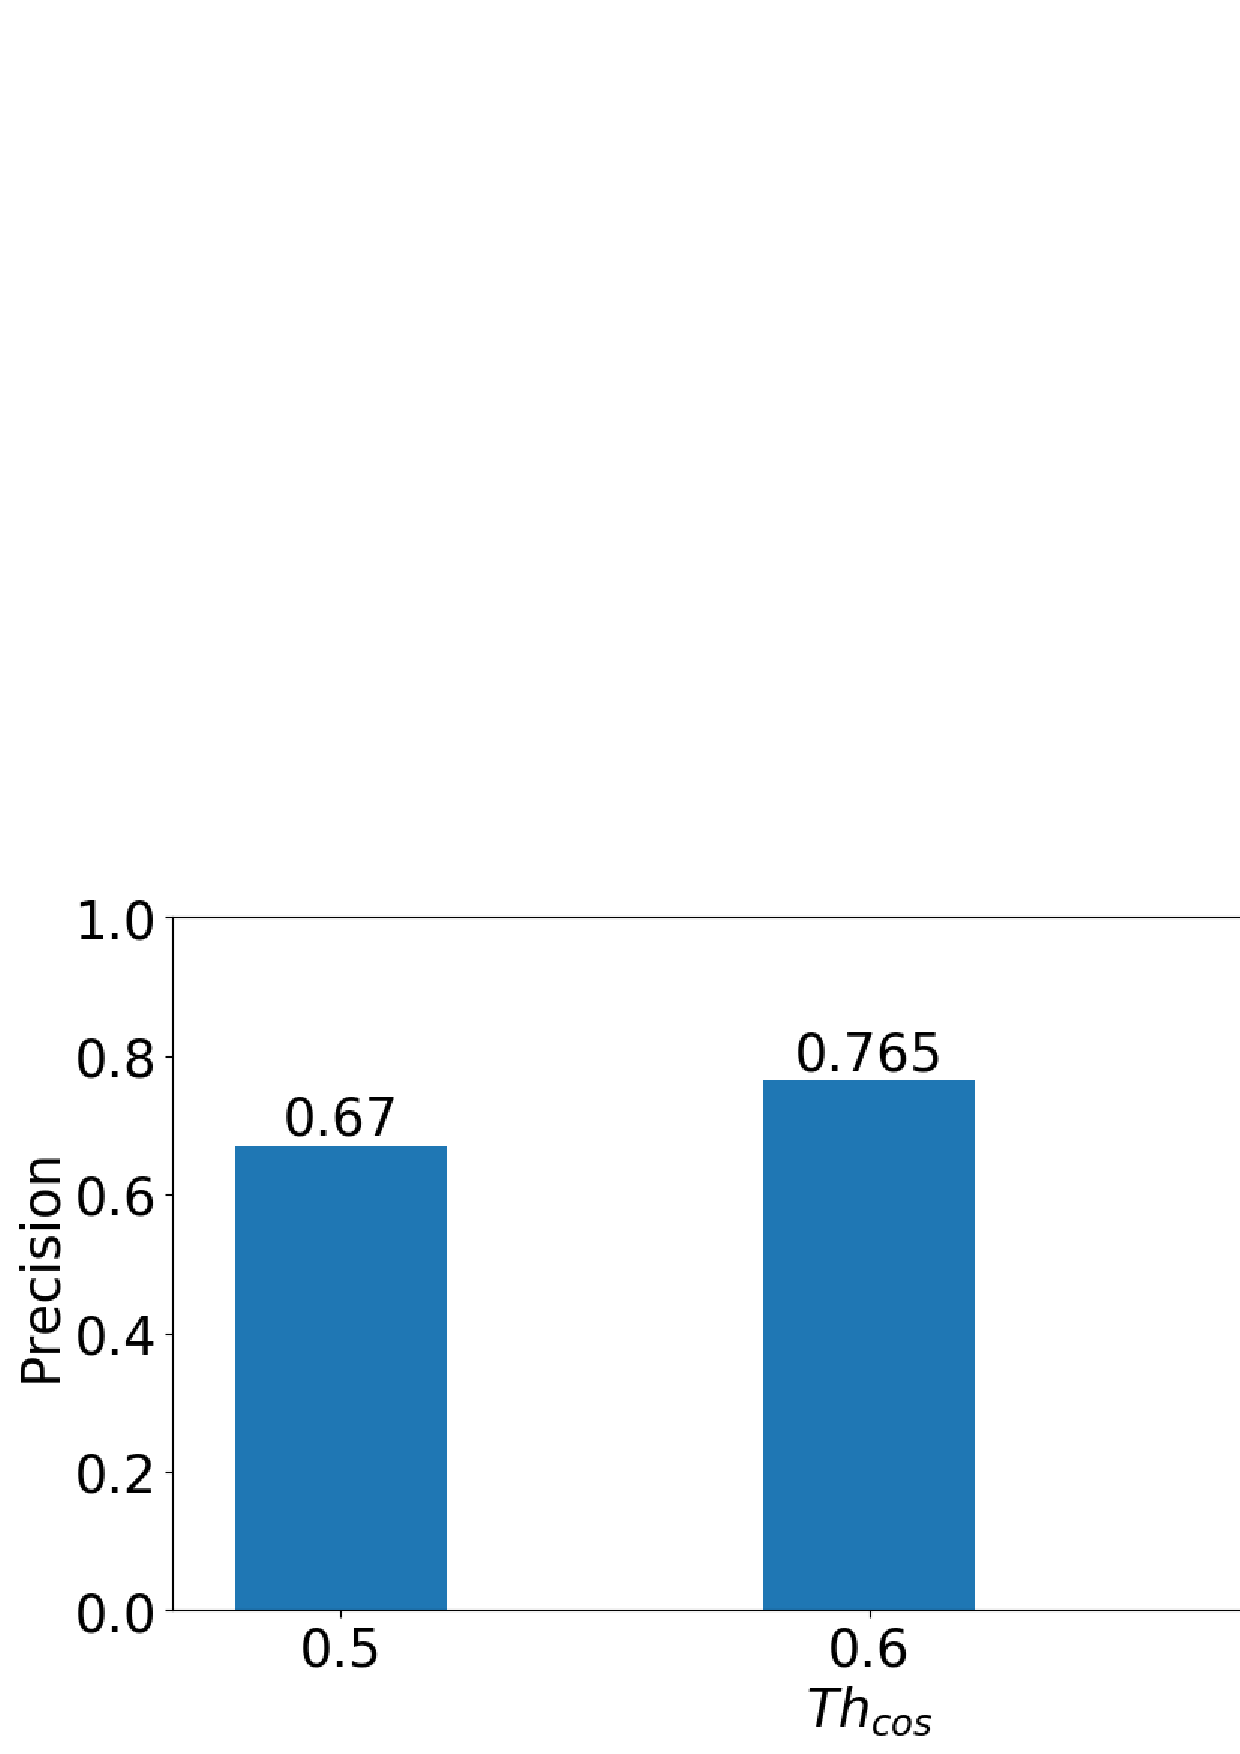
\includegraphics[keepaspectratio, scale=0.25]
                          {./figure/baseline_p.eps}}
      \end{minipage} \\

      \begin{minipage}{0.06\hsize}
        \vspace{5mm}
      \end{minipage} \\
 
 
%----- fmeasure -----
 
      \begin{minipage}{0.40\hsize}
        \centering
          \subfigure[F-measure]{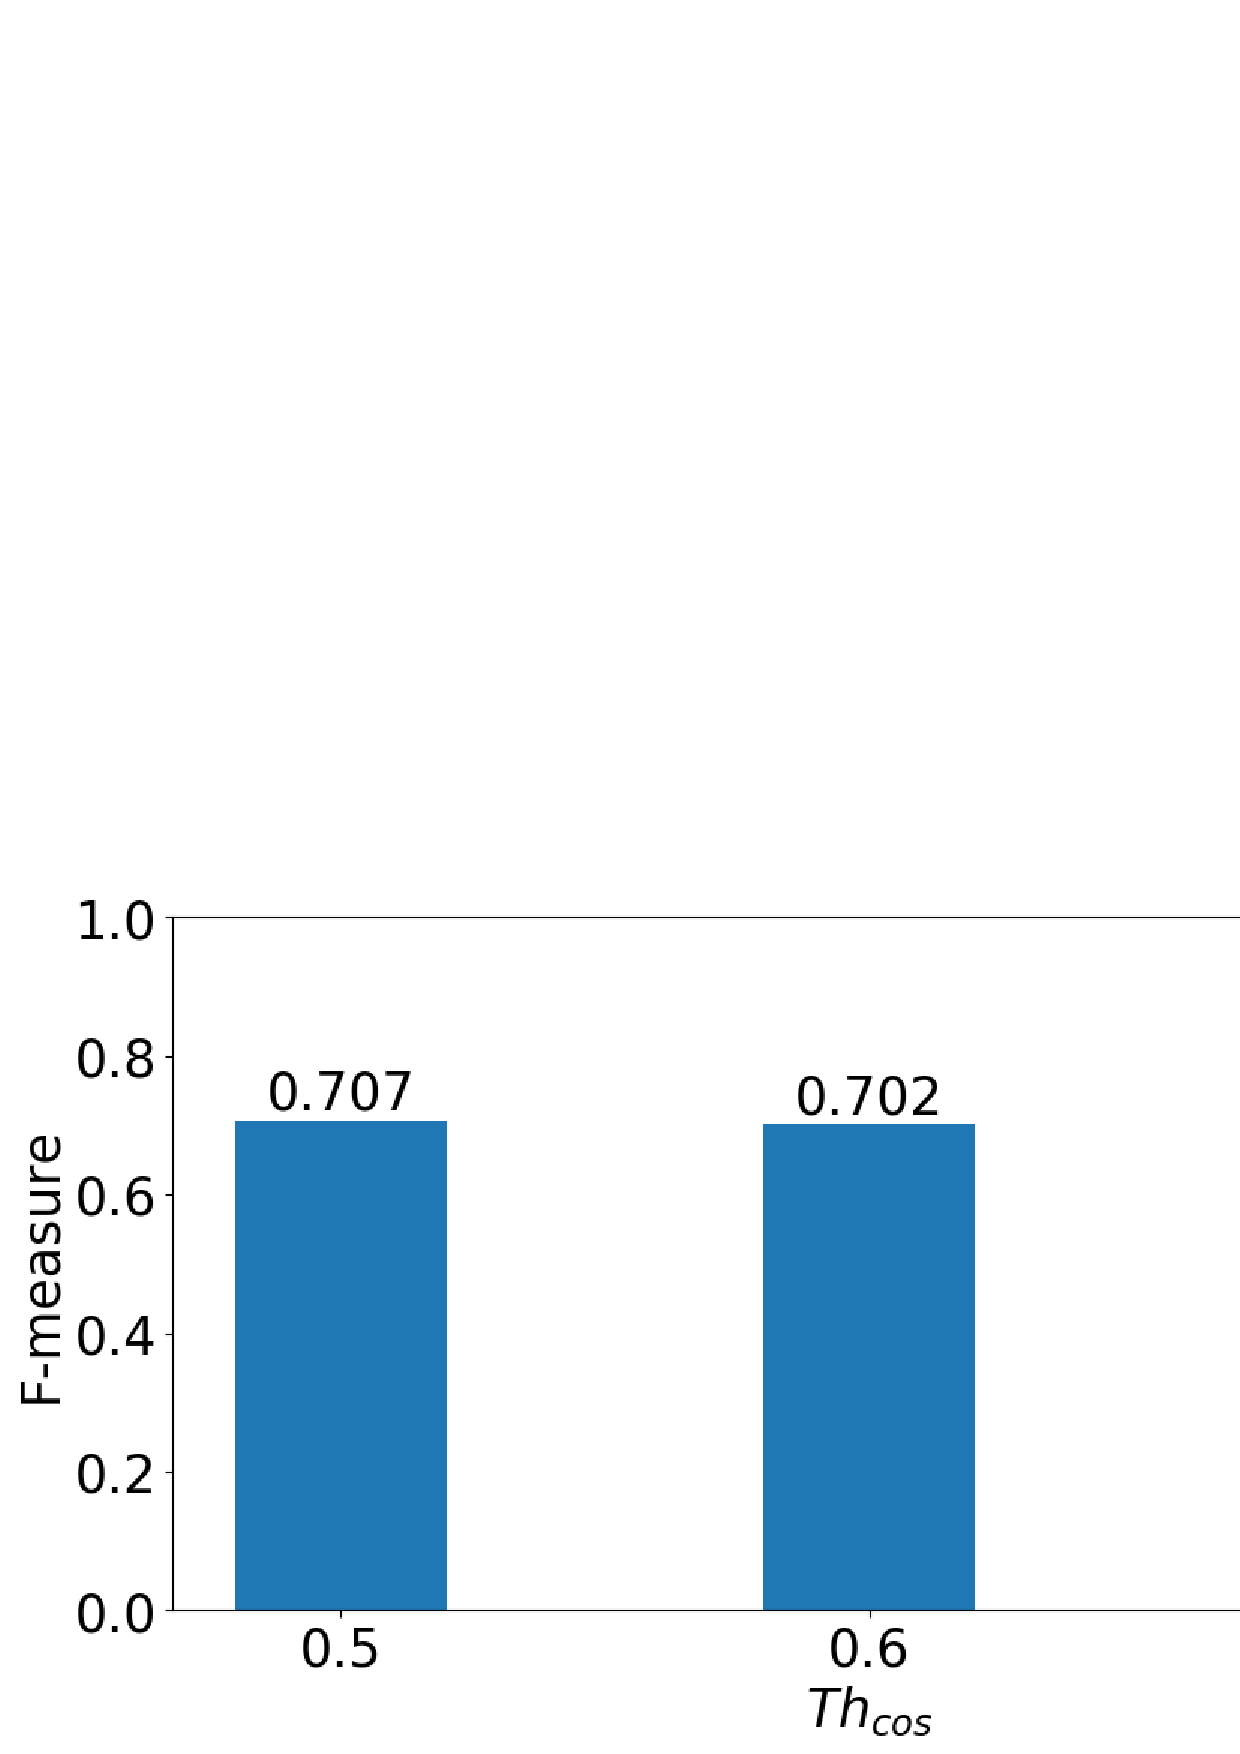
\includegraphics[keepaspectratio, scale=0.25]
                          {./figure/baseline_f.eps} \label{baseline_fmeasure}}
      \end{minipage}

      \begin{minipage}{0.06\hsize}
        \hspace{0.5mm}
      \end{minipage}


    \end{tabular}
\caption{Baseline2による発話区間検出精度 \label{fig:result_anchor_baseline}}
\end{figure} 


\begin{table}[H]
  \begin{center}
    \caption{Baseline2による各ニュース番組音声のニュースアンカーの発話検出精度($Th_{cos}=0.5$) \label{table:baseline_eachnews}}
    \begin{tabular}{|c||c|c|c|c|} \hline
データID & Recall & Precision & F-meature & 作成したクラスタ数\\ \hline
ニュース1 & 0.970 & 0.623 & 0.758 & 1 \\ \hline
ニュース2 & 0.709 & 0.437 & 0.540 & 2 \\ \hline
ニュース3 & 0.736 & 0.719 & 0.727 & 2 \\ \hline
ニュース4 & 0.728 & 0.661 & 0.693 & 2 \\ \hline
ニュース5 & 0.683 & 0.947 & 0.793 & 2 \\ \hline
計 & 0.748 & 0.670 & 0.707 &  \\ \hline
    \end{tabular}
  \end{center}
\end{table}

%手法1の図
\begin{figure}[H]
  \centering
    \begin{tabular}{c}
 
%----- recall -----
 
      \begin{minipage}{0.40\hsize}
        \centering
          \subfigure[Recall]{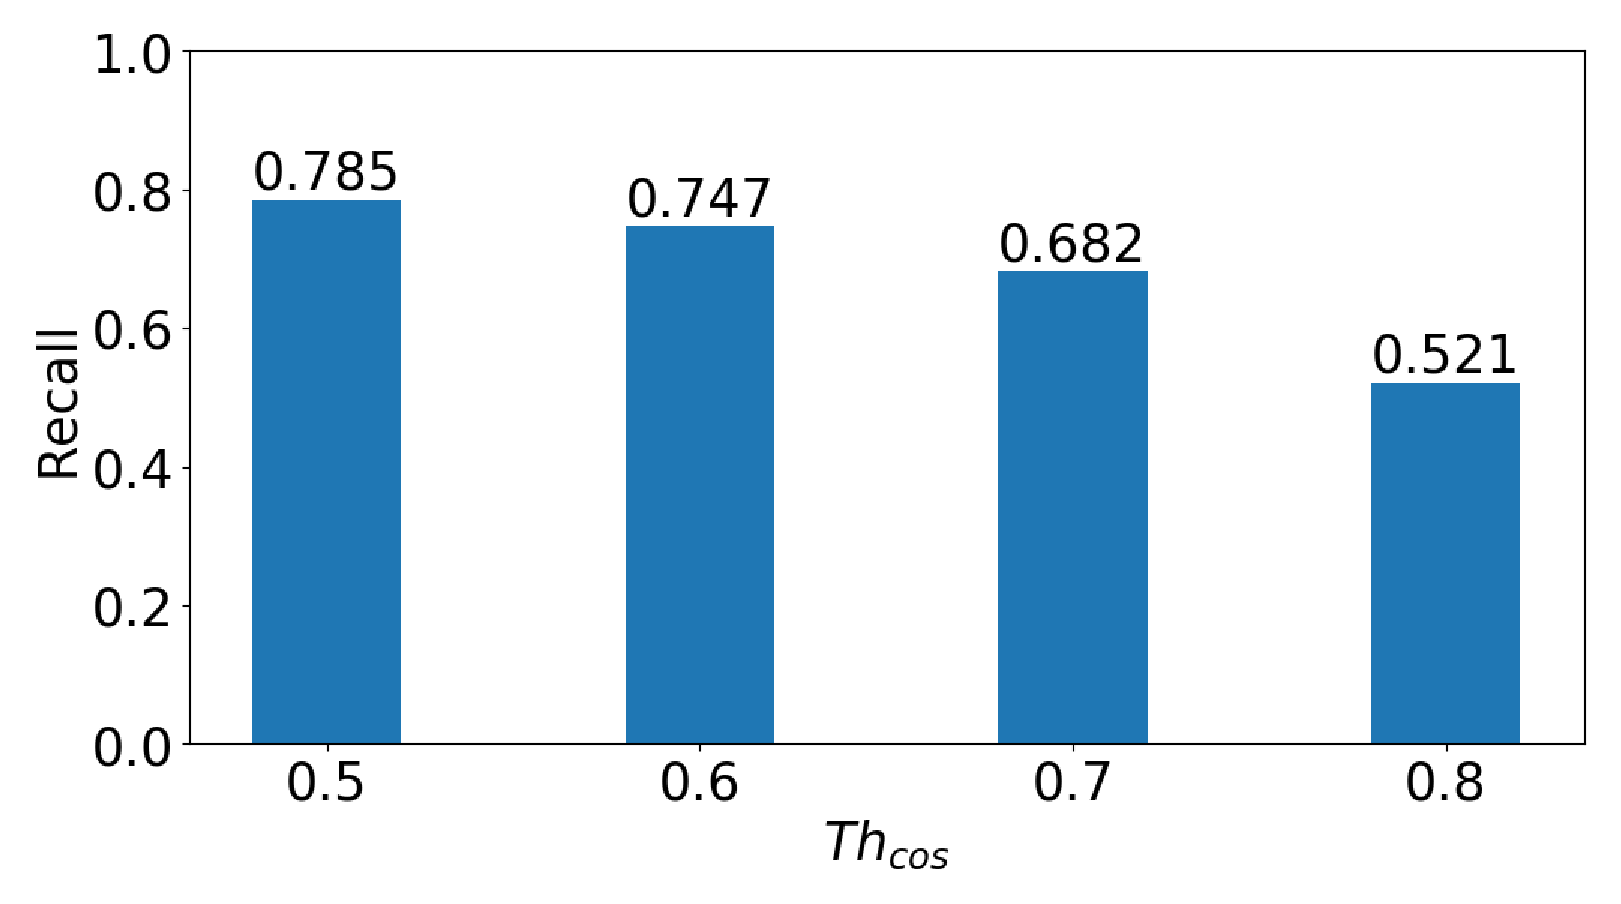
\includegraphics[keepaspectratio, scale=0.25]
                          {./figure/prob1_12_r.eps}}
      \end{minipage}

      \begin{minipage}{0.06\hsize}
        \hspace{0.5mm}
      \end{minipage}
 
%----- precision -----
 
      \begin{minipage}{0.40\hsize}
        \centering
          \subfigure[Precision]{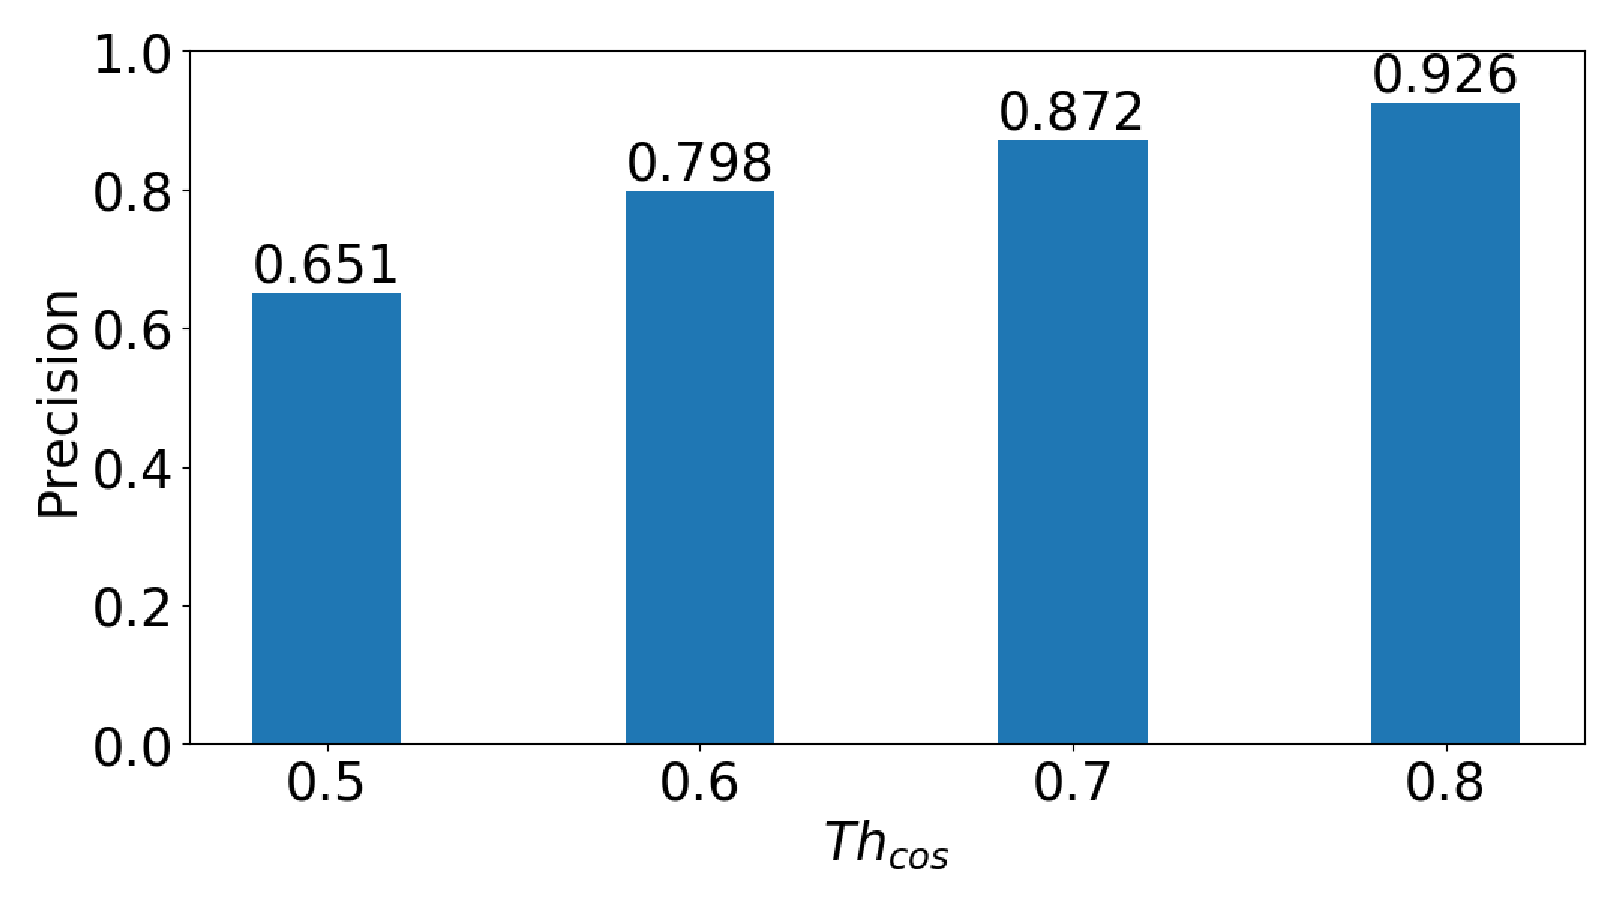
\includegraphics[keepaspectratio, scale=0.25]
                          {./figure/prob1_12_p.eps}}
      \end{minipage} \\

      \begin{minipage}{0.06\hsize}
        \vspace{5mm}
      \end{minipage} \\
 
 
%----- fmeasure -----
 
      \begin{minipage}{0.40\hsize}
        \centering
          \subfigure[F-measure]{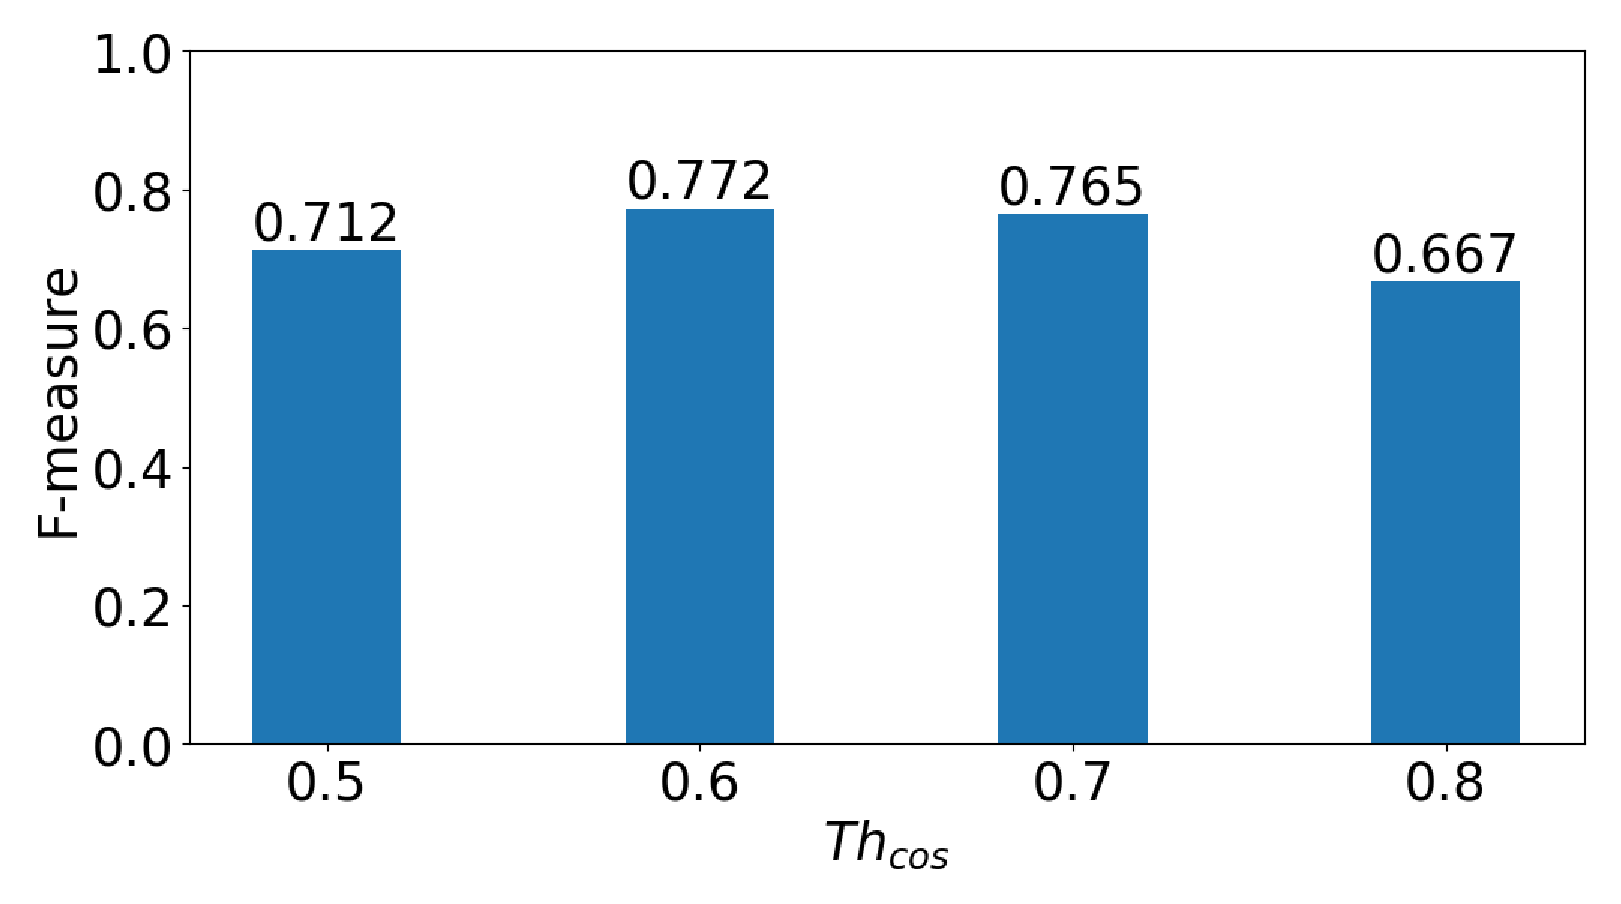
\includegraphics[keepaspectratio, scale=0.25]
                          {./figure/prob1_12_f.eps} \label{prob1_fmeasure}}
      \end{minipage}

      \begin{minipage}{0.06\hsize}
        \hspace{0.5mm}
      \end{minipage}
 

    
    \end{tabular}
\caption{手法1によるアンカーの発話区間検出精度 ($Th_{time}=1.2$) \label{fig:result_anchor_prob1}}
\end{figure} 

\begin{table}[H]
  \begin{center}
    \caption{手法1による各ニュース番組音声のニュースアンカーの発話検出精度($Th_{cos}=0.6,Th_{time}=1.2$) }
    \begin{tabular}{|c||c|c|c|c|} \hline
データID & Recall & Precision & F-meature & 作成したクラスタ数\\ \hline
ニュース1 & 0.964 & 0.707 & 0.815 & 1 \\ \hline
ニュース2 & 0.764 & 0.685 & 0.722 & 2 \\ \hline
ニュース3 & 0.729 & 0.860 & 0.789 & 2 \\ \hline
ニュース4 & 0.683 & 0.741 & 0.711 & 2 \\ \hline
ニュース5 & 0.695 & 0.978 & 0.813 & 2 \\ \hline
計 & 0.747 & 0.798 & 0.765 &  \\ \hline
    \end{tabular}
  \end{center}
\end{table}

%手法2の図
\begin{figure}[H]
  \centering
    \begin{tabular}{c}
 
%----- recall -----
 
      \begin{minipage}{0.40\hsize}
        \centering
          \subfigure[Recall]{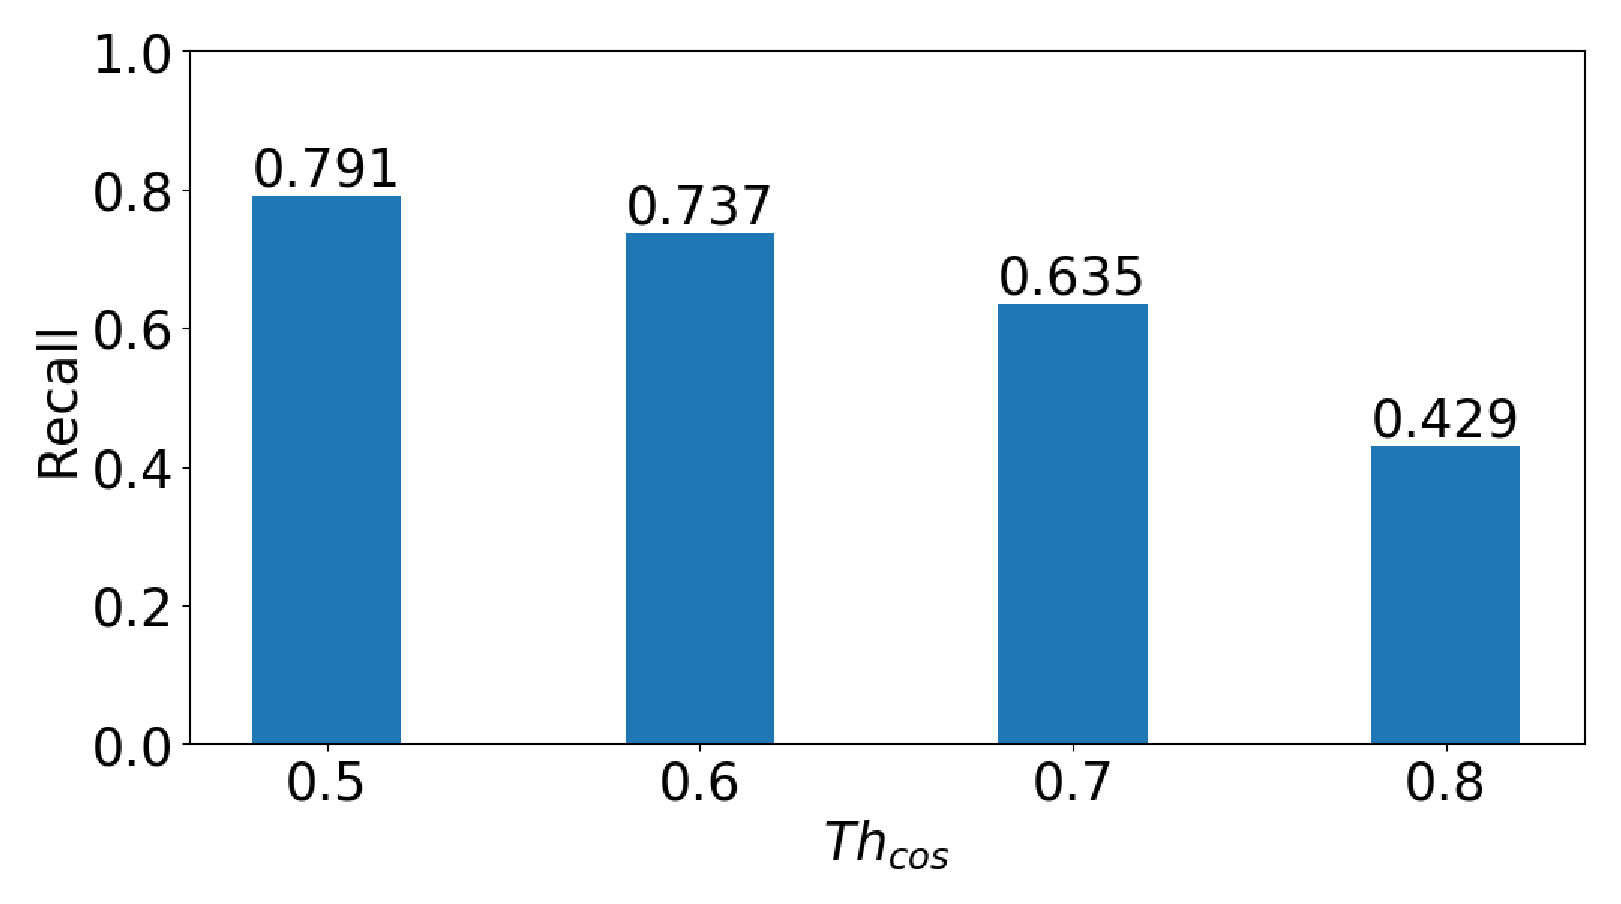
\includegraphics[keepaspectratio, scale=0.25]
                          {./figure/prob2_r.eps}}
      \end{minipage}

      \begin{minipage}{0.06\hsize}
        \hspace{0.5mm}
      \end{minipage}
 
%----- precision -----
 
      \begin{minipage}{0.40\hsize}
        \centering
          \subfigure[Precision]{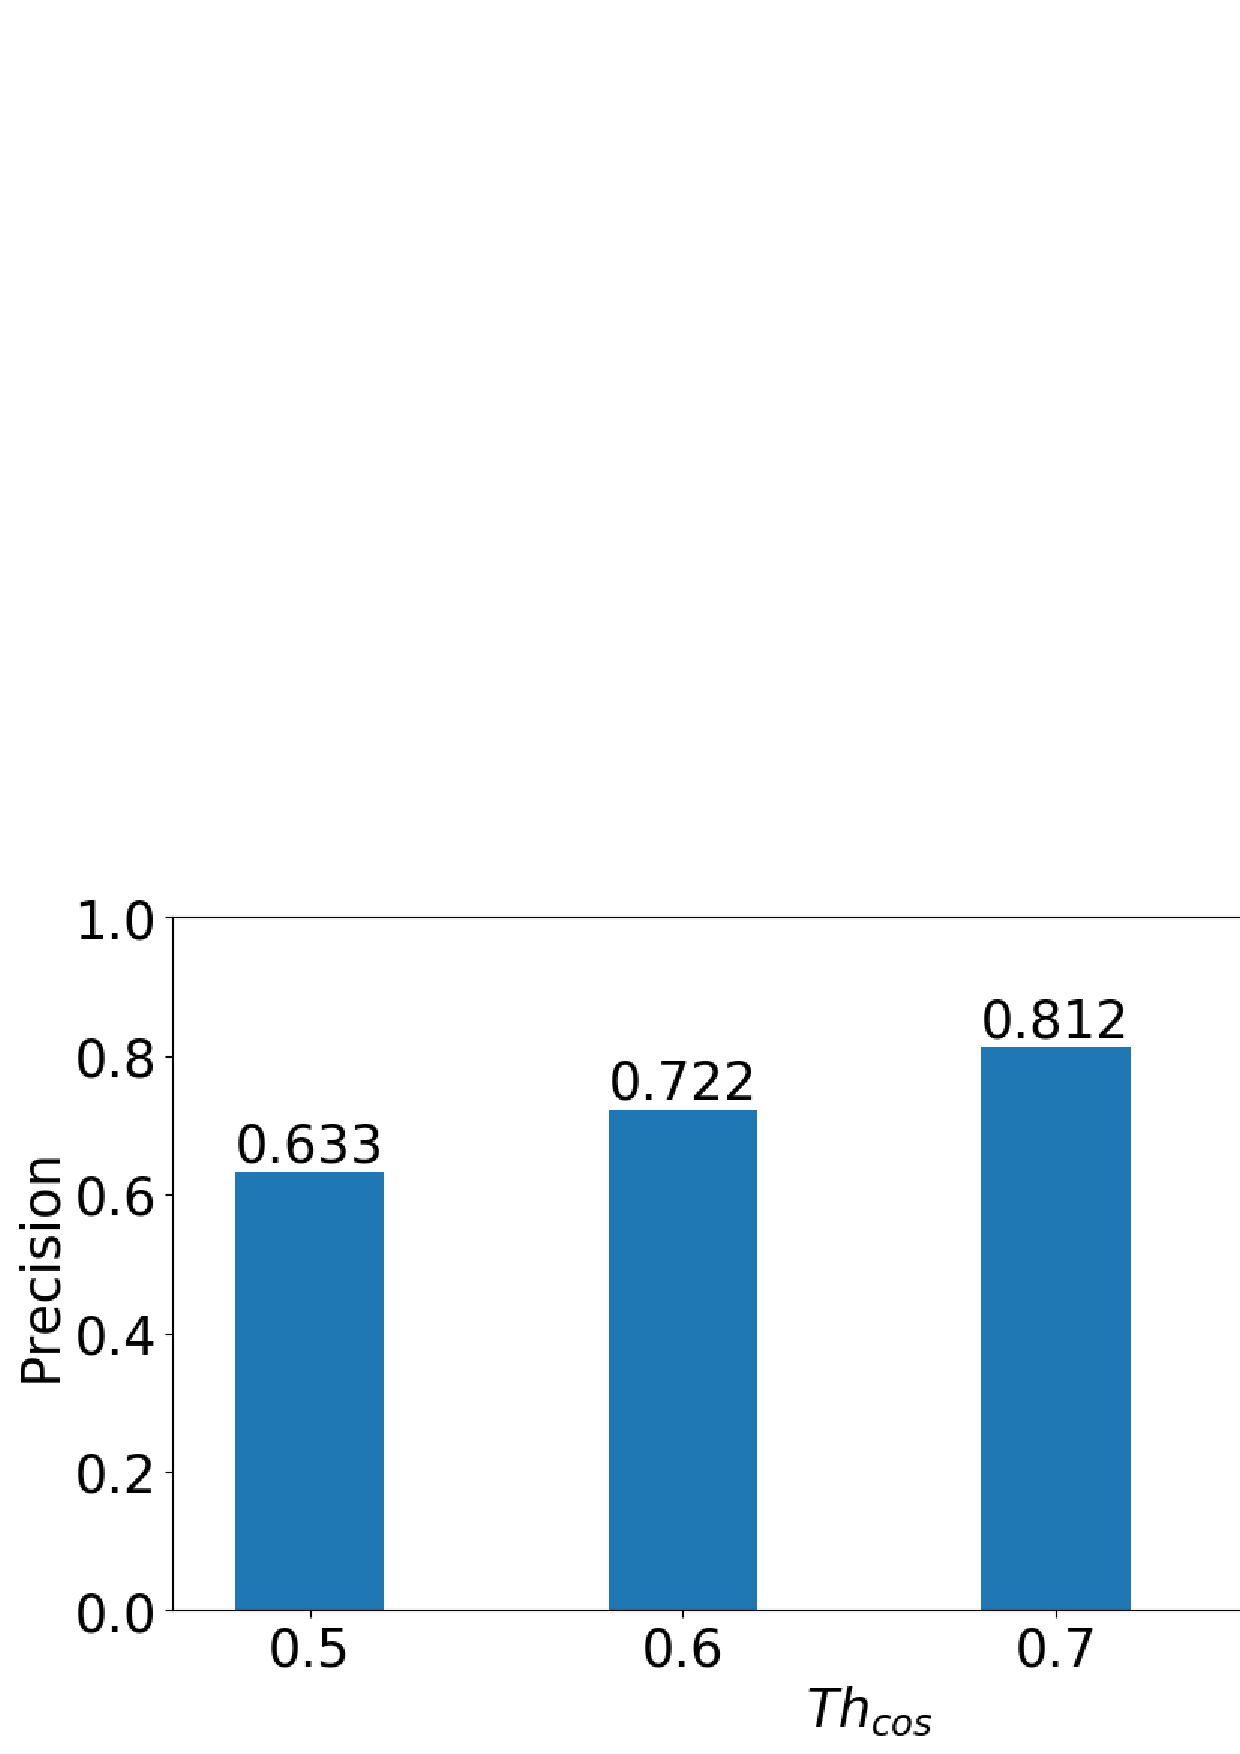
\includegraphics[keepaspectratio, scale=0.25]
                          {./figure/prob2_p.eps}}
      \end{minipage} \\

      \begin{minipage}{0.06\hsize}
        \vspace{5mm}
      \end{minipage} \\
 
 
%----- fmeasure -----
 
      \begin{minipage}{0.40\hsize}
        \centering
          \subfigure[F-measure]{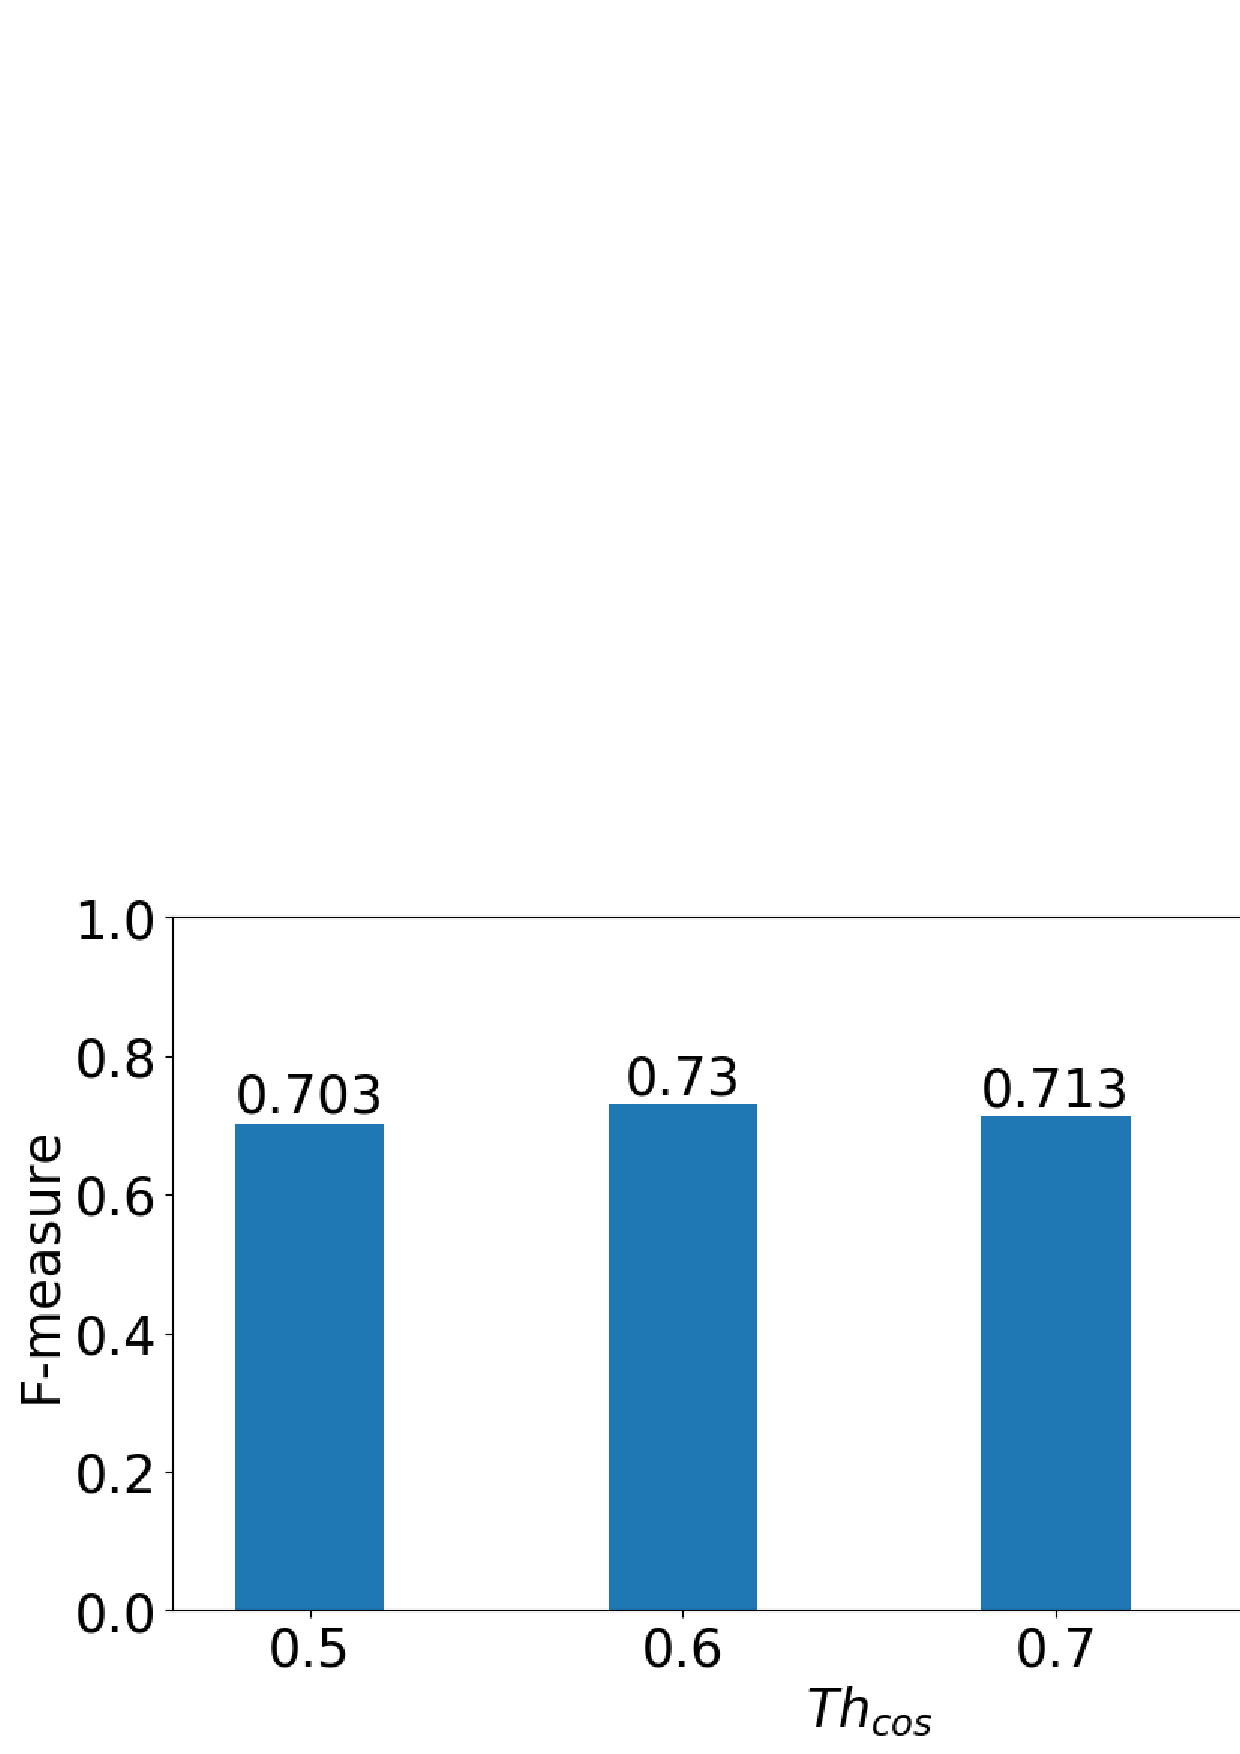
\includegraphics[keepaspectratio, scale=0.25]
                          {./figure/prob2_f.eps} \label{prob2_fmeasure}}
      \end{minipage}

      \begin{minipage}{0.06\hsize}
        \hspace{0.5mm}
      \end{minipage}
 
    \end{tabular}
\caption{手法2によるニュースアンカーの発話検出精度 \label{fig:result_anchor_prob2}}
\end{figure} 

\begin{table}[H]
  \begin{center}
    \caption{手法2による各ニュース番組音声のニュースアンカーの発話検出精度($Th_{cos}=0.6$) }
    \begin{tabular}{|c||c|c|c|c|} \hline
データID & Recall & Precision & F-meature & 作成したクラスタ数\\ \hline
ニュース1 & 0.958 & 0.617 & 0.751 & 1 \\ \hline
ニュース2 & 0.788 & 0.512 & 0.621 & 2 \\ \hline
ニュース3 & 0.695 & 0.823 & 0.754 & 2 \\ \hline
ニュース4 & 0.683 & 0.732 & 0.707 & 2 \\ \hline
ニュース5 & 0.679 & 0.960 & 0.796 & 2 \\ \hline
計 & 0.737 & 0.722 & 0.730 &  \\ \hline
    \end{tabular}
  \end{center}
\end{table}

%手法3の図
\begin{figure}[H]
  \centering
    \begin{tabular}{c}
 
%----- recall -----
 
      \begin{minipage}{0.40\hsize}
        \centering
          \subfigure[Recall]{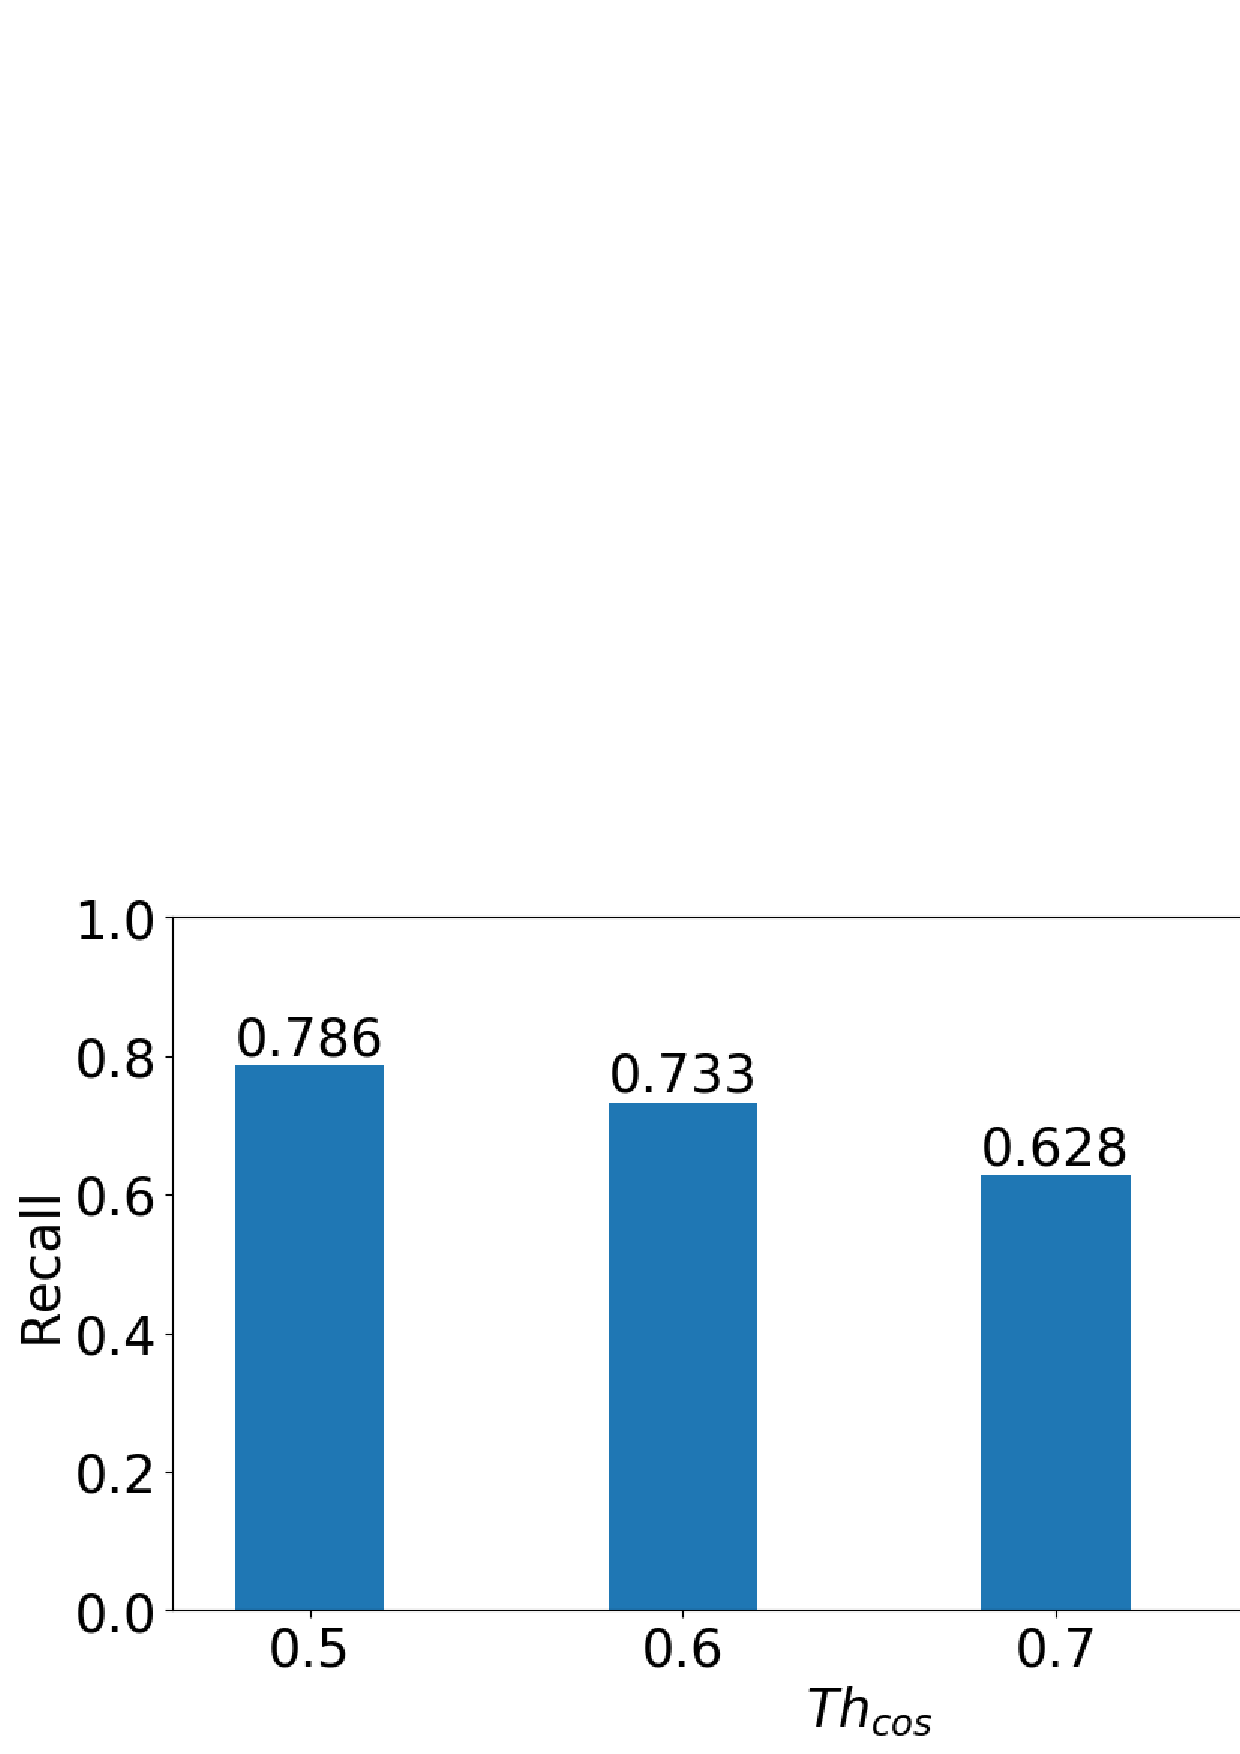
\includegraphics[keepaspectratio, scale=0.25]
                          {./figure/prob3_11_r.eps}}
      \end{minipage}

      \begin{minipage}{0.06\hsize}
        \hspace{0.5mm}
      \end{minipage}
 
%----- precision -----
 
      \begin{minipage}{0.40\hsize}
        \centering
          \subfigure[Precision]{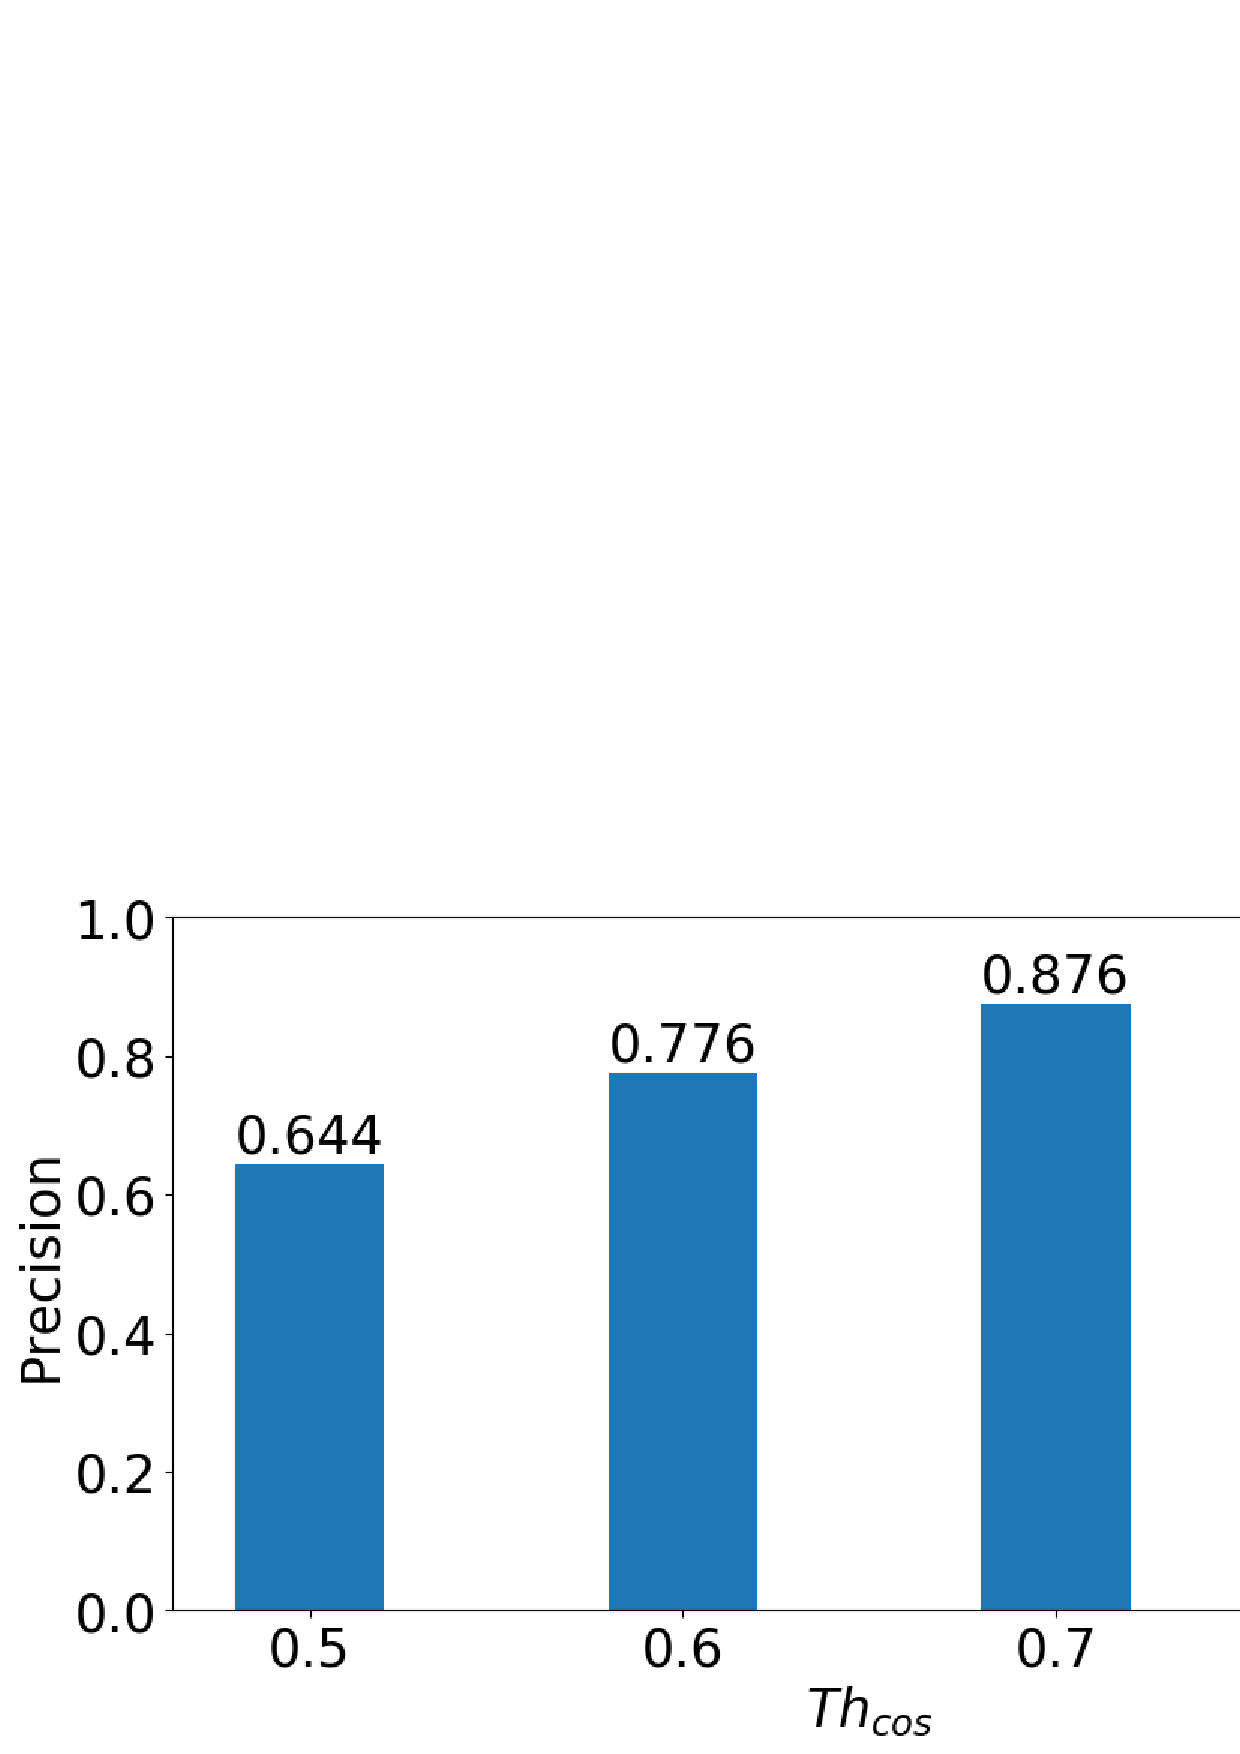
\includegraphics[keepaspectratio, scale=0.25]
                          {./figure/prob3_11_p.eps}}
      \end{minipage} \\

      \begin{minipage}{0.06\hsize}
        \vspace{5mm}
      \end{minipage} \\
 
 
%----- fmeasure -----
 
      \begin{minipage}{0.40\hsize}
        \centering
          \subfigure[F-measure]{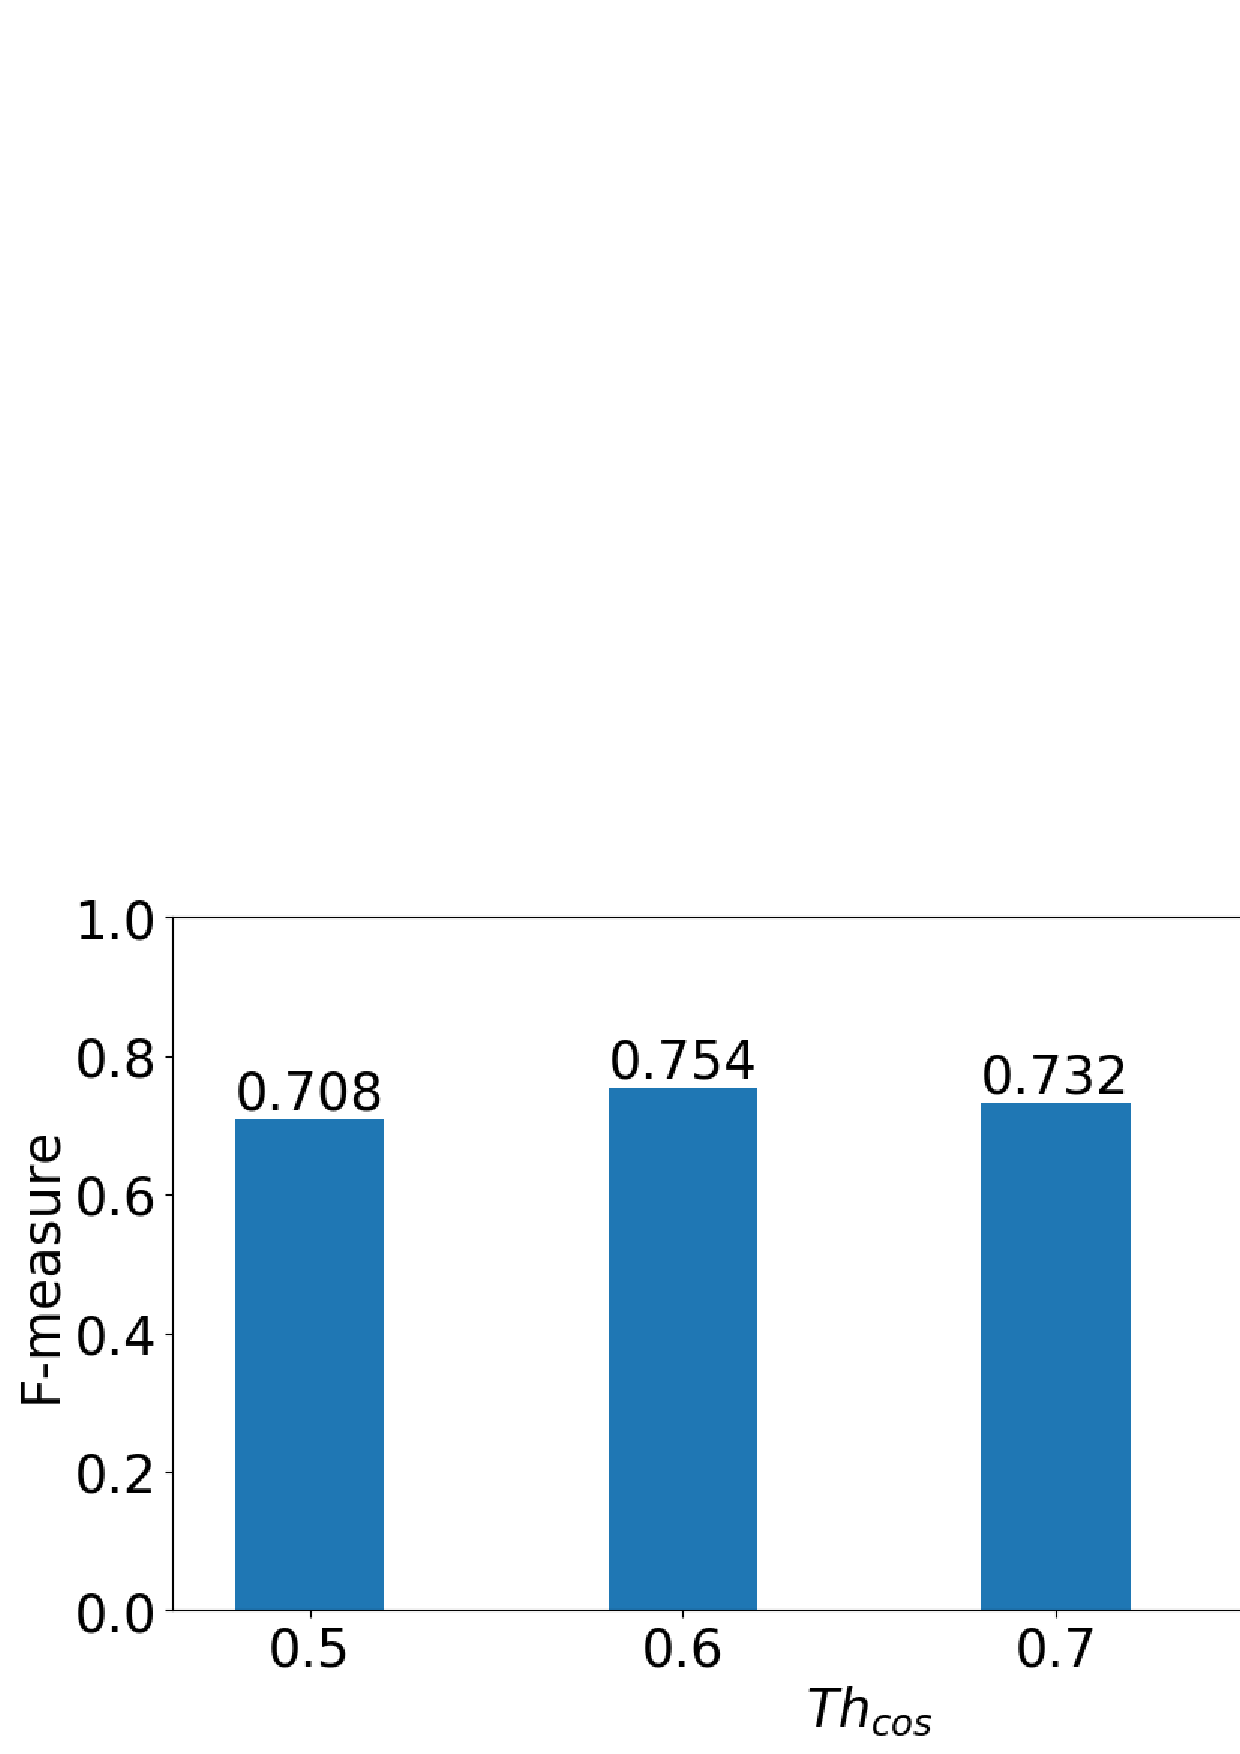
\includegraphics[keepaspectratio, scale=0.25]
                          {./figure/prob3_11_f.eps} \label{prob3_fmeasure}}
      \end{minipage}

      \begin{minipage}{0.06\hsize}
        \hspace{0.5mm}
      \end{minipage}
 
%----- acc time -----
\begin{comment}
      \begin{minipage}{0.40\hsize}
        \centering
          \subfigure[$Acc_{time}$]{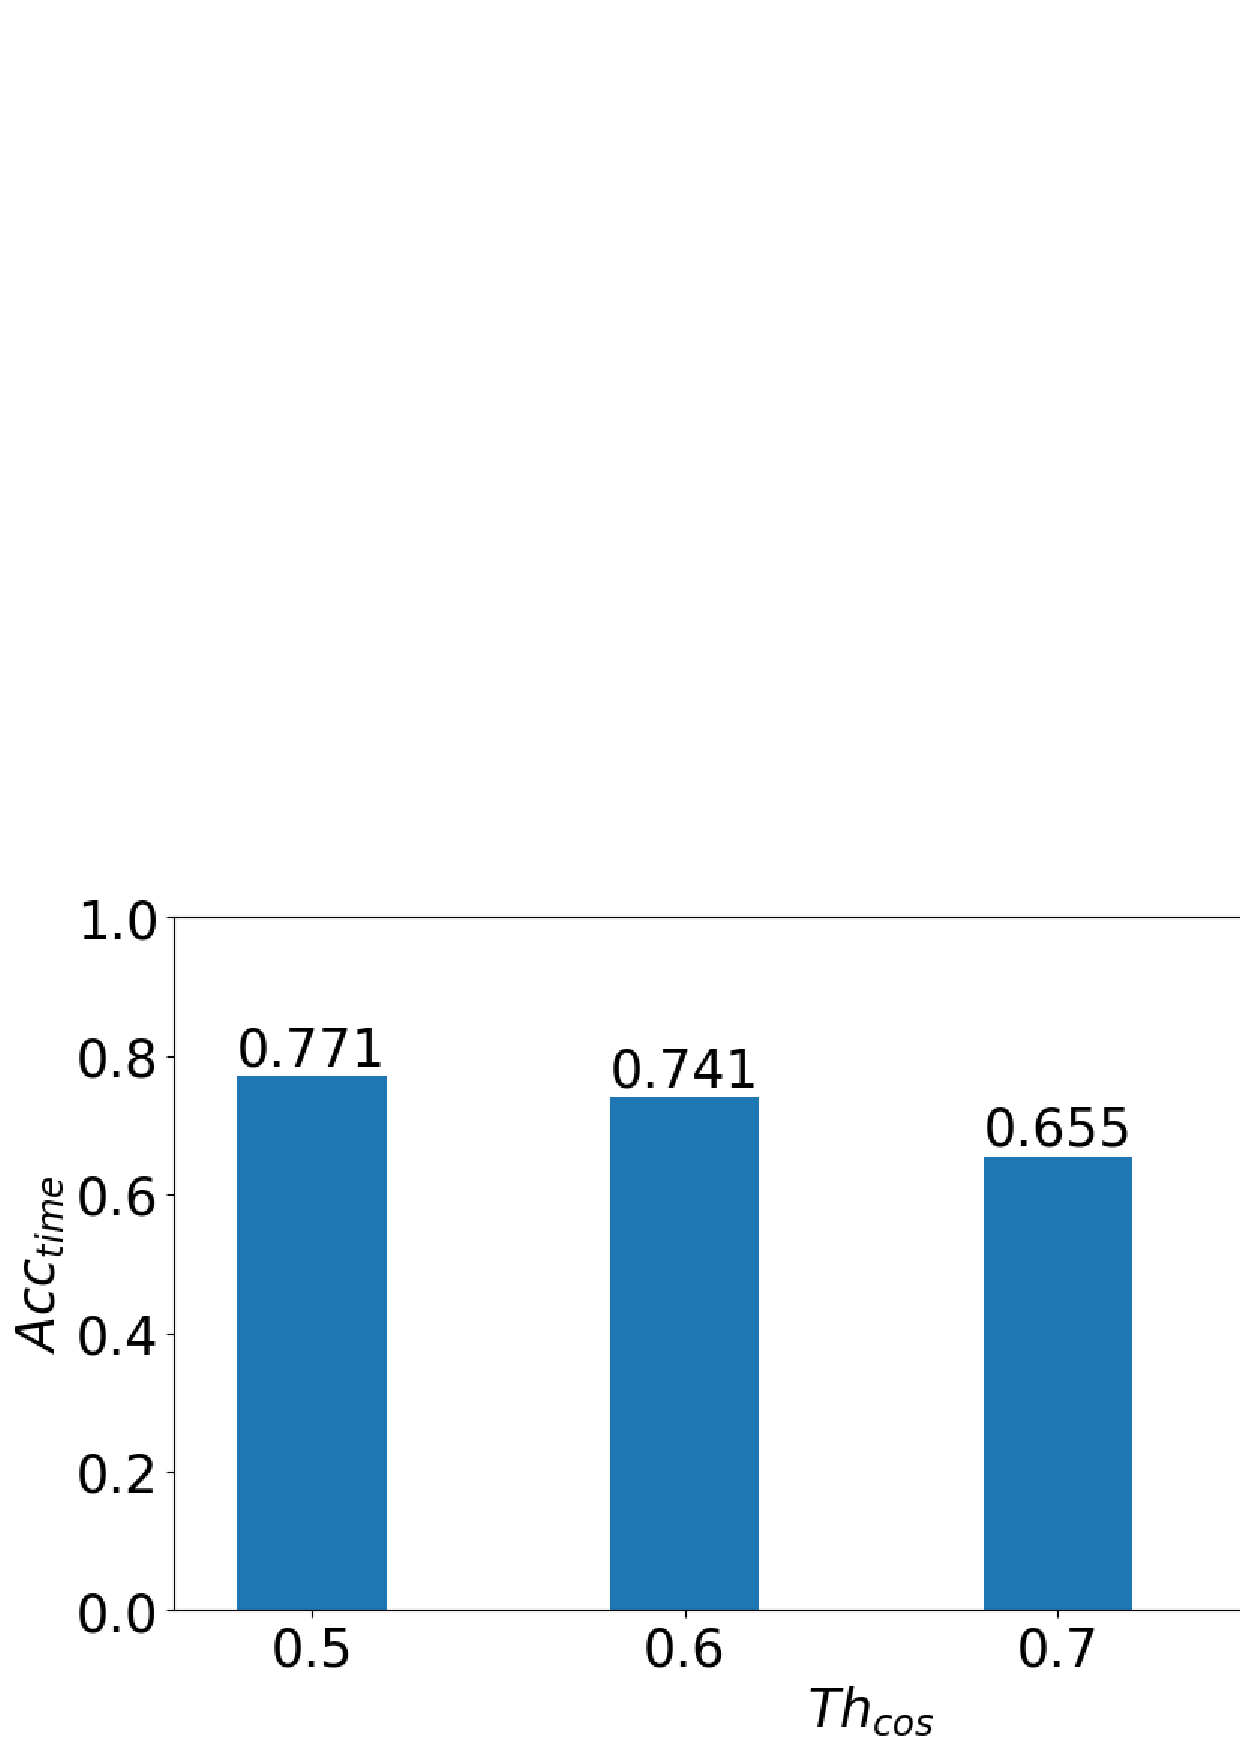
\includegraphics[keepaspectratio, scale=0.25]
                          {./figure/prob3_11_acc.eps}}
      \end{minipage}
\end{comment}
    \end{tabular}
\caption{手法3によるアンカーの発話区間検出精度 ($Th_{time}=1.1$) \label{fig:result_anchor_prob3}}
\end{figure} 


\begin{table}[H]
  \begin{center}
    \caption{手法3による各ニュース番組音声のニュースアンカーの発話検出精度($Th_{cos}=0.6,Th_{time}=1.1$) \label{table:prob3_eachnews}}
    \begin{tabular}{|c||c|c|c|c|} \hline
データID & Recall & Precision & F-meature & 作成したクラスタ数\\ \hline
ニュース1 & 0.958 & 0.702 & 0.810 & 1 \\ \hline
ニュース2 & 0.758 & 0.590 & 0.663 & 2 \\ \hline
ニュース3 & 0.725 & 0.846 & 0.781 & 2 \\ \hline
ニュース4 & 0.646 & 0.755 & 0.696 & 2 \\ \hline
ニュース5 & 0.683 & 0.973 & 0.802 & 2 \\ \hline
計 & 0.733 & 0.776 & 0.754 &  \\ \hline
    \end{tabular}
  \end{center}
\end{table}

実験の結果、Baseline2を各手法を比較したとき、ニュースアンカーの検出精度の指標であるF-measureが手法1では6.5\%(図\ref{prob1_fmeasure})、手法2では2.3\%(図\ref{prob2_fmeasure})、手法3では4.7\%(図\ref{prob3_fmeasure})の向上が確認された。また、Baselineと提案手法の全てにおいてニュース2の検出精度であるPrecisionが最も低い。\par
いずれの手法においても$Th_{cos}$が小さい時にはRecallが高く、大きい時にはPrecisionが高くなる傾向が確認された。また、$Acc_{time}$は$Th_{cos}$が大きくなると低くなる傾向にある。また、Baseline1を除く全ての手法でニュースアンカーの人数と検出したニュースアンカーの人数が同じであった。\par

\vspace{0.2in}\noindent{\textbf{\underline{ニュースアンカーとして検出した発話の時間による評価}}}\par

\section{考察}
Baselineと提案手法を比較したとき提案手法のニュースアンカーの発話検出精度が最大で6.5\%向上したことから、結合した発話区間から抽出したi-vectorをニュースアンカーの検出に用いることは有効であることを示した。これは、提案手法では発話の時間間隔、発話環境を考慮して結合した発話区間からi-vectorを抽出したことで、従来と比較してi-vectorが話者の特徴を表現できたためであると考えられる。また、Baselineにおいて、$Th_{cos}$が0.8のとき、提案手法のみニュースアンカーの発話検出を行うことが出来たことから、i-vectorの抽出精度が向上したと考えることができる。\par
手法2と手法3の検出精度のF-measureが手法1と比較して低下した理由として、ニュースアンカーの発話中に流れるVTRの存在が挙げられる。話者が切り替わっていない場合であってもVTRに含まれる雑音や音楽が同時に流れることによって発話環境の変化と誤識別したため、発話区間の結合ができなかったためであると考えられる。\par
いずれの手法でもニュース2のニュースアンカーの発話検出精度であるP値が他のニュースと比較して低い理由として、表\ref{table:test_detail}や表\ref{table:num_of_anchor}で示されているように、アンカーの発話の割合が少ないことが挙げられる。本研究で用いたニュースアンカーの発話検出手法\cite{nozaki_gakuseikai}は、ニュースアンカーの発話の割合が多いことに着目して検出を行っている。そのため、ニュースアンカー以外の発話が多い話者の発話をニュースアンカーとして誤識別したためPrecisionが低下したと考えられる。\par
今後、発話数が少ないニュースアンカーの発話検出手法を検討することで、さらなるニュースアンカーの発話検出精度の向上が期待できると考えられる。\par
\begin{comment}
また、ニュースアンカーの発話検出精度の向上における音声認識への効果を検証するために、検出されたニュースアンカーの発話の音声認識実験を行った。音声認識システムの概要、実験の詳細を付録\ref{chapter:speech_recog}に記載する。音声認識実験の結果、インデクシングに十分な精度で音声認識が行われたとは言えないため、音声認識精度向上のために雑音除去や雑音に頑健な音声認識システムを構築する必要があると考えられる。
\end{comment}
